\chapter{Case study 2: Creating new constraints}
\label{chap:case_study2}

Chapter \ref{chap:case_study1} showcased the motivation and the general capabilities of my project but did not show actual DSL scripts, because the \nameref{chap:konst_dsl} chapter was a prerequisite for that. This chapter will continue the case study, demonstrating how to write scripts in my DSL. Initially, I'll show how to write a report, followed by an example of writing a webhook for the same policy. Lastly, I'll introduce an advanced use case to showcase the robust error-handling features of my platform.

\section{Creating a report}

Let's consider a very simple policy: `All images must come from the internal company registry.' To enforce this, we'll start by detecting which pods violate this policy. Create a new file using the template from the \ref{code:server_boilerplate} code snippet. Add a report block with an aggregation group on the pods. The \ref{code:c2_1} code snippet shows how it should look.

\begin{minipage}{\linewidth}
\begin{lstlisting}[caption={Report skeleton},language=Kotlin,label=code:c2_1]
package me.btieger

import me.btieger.dsl.*

const val companyPrefix = "tiegris/"
val companPolicies = server("company-policies") {
  report {
    aggregation("Pods", kubelist { pods() }) {
  
    }
  }
}
\end{lstlisting}
\end{minipage}

To determine whether all the containers of a pod are using images only from the company registry, we need to express this requirement with mathematical precision using first-order logic. Here are two continuous sentences that express the requirement:

`Tag the pod if any of its container's images do not start with the company prefix.'

`Do not tag the pod, if all of its container's images start with the company prefix.'

The \ref{code:c2_2} code snippet demonstrates how to implement the first expression in code.

\begin{minipage}{\linewidth}
\begin{lstlisting}[caption={Tag pods},language=Kotlin,label=code:c2_2]
aggregation("Pods", kubelist { pods() }) {
  tag("Image not from company registry") {
    item.spec.containers.any { !it.image.startsWith(companyPrefix) }
  }
}
\end{lstlisting}
\end{minipage}

The script retrieves the list of pods from the Kubernetes API, but to do that successfully, it needs authorization. To achieve this, we need to associate a \emph{ClusterRole} with the agent. In the demo files, there is a \emph{ClusterRole} definition in the readPods.yaml file (\ref{appendix:csr:readpods}). We want our agent to be least privileged, so we are only giving it read access to the pods with the \emph{read-pods} \emph{ClusterRole}.

The \ref{code:c2_3} code snippet shows the final script. After creating the \emph{read-pods} \emph{ClusterRole} with the \lstinline|kubectl apply -f <filename>| command and deploying the script, we should observe the same report as shown in the \ref{fig:report} figure.

\begin{lstlisting}[caption={Final reporting script},language=Kotlin,label=code:c2_3]
package me.btieger
import me.btieger.dsl.*

const val companyPrefix = "tiegris/"
val companyPolicies = server("company-policies") {
  clusterRole = "read-pods"
  report {
    aggregation("Pods", kubelist { pods() }) {
      tag("Image not from company registry") {
        item.spec.containers.any { !it.image.startsWith(companyPrefix) }
      }
    }
  }
}
\end{lstlisting}

\begin{figure}[h]
  \centering
  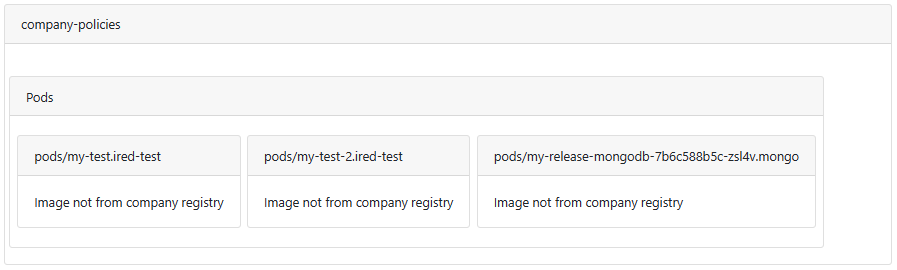
\includegraphics[width=150mm, keepaspectratio]{content/60_caseStudy2/company_policies_1.png}
  \caption{Report generated by the script}
  \label{fig:report}
\end{figure}

The report shows that there are 3 pods, which use images outside from the company registry.

\clearpage
\section{Creating a webhook}

Now, let's move on to the enforcement aspect. Utilizing the description provided in Section \ref{sec:webhooks}, we can develop this segment of the script. The only non-trivial consideration is determining the type of events to intercept. We aim to capture user actions rather than controller resource actions. Therefore, we should specifically monitor the creation of deployments, stateful sets, and daemon sets, instead of just pod creations. To be more precise, we could extend our monitoring to include various resources that can create pods, including pod creations, but for the purpose of this demo, we'll keep it simple.

The code snippet in \ref{code:c2_4} illustrates this webhook. It is designed to listen for the creation and updates of deployment, statefulset, and daemonset resources across any namespace. It permits these actions only if all Docker images within their pod's containers start with the company prefix; otherwise, it returns a descriptive error message.

\begin{lstlisting}[caption={Company policy enforcer webhook},language=Kotlin,label=code:c2_4]
webhook("only-internal-registry") {
  operations(CREATE, UPDATE)
  apiGroups(APPS)
  apiVersions(ANY)
  resources(DEPLOYMENTS, STATEFULSETS, DAEMONSETS)
  namespaceSelector { }
  failurePolicy(FAIL)
  behavior {
    allowed {
      podSpec!!.containers.all { it.image.startsWith(companyPrefix) }
    }
    status {
      message = "All images must be from the company registry."
    }
  }
}
\end{lstlisting}

If we incorporate the webhook from the code snippet in \ref{code:c2_4} into the script and redeploy it, we can observe it in action. Execute the following command from the correct directory: \lstinline|kubectl create ns policy-test && kubectl apply -f k8s/test-policy.yaml -n policy-test|

This command creates a test \emph{Pod} (see \ref{appendix:csr:testpolicy}) with a container using a Docker image from Docker Hub. In response, we should encounter the following error message: `Error from server: error when creating "k8s/test-policy.yaml": admission webhook "only-internal-registry.btieger.me" denied the request: All images must be from the company registry.'

If we modify the image to, for example, `tiegris/apples-users' and redeploy the \emph{Pod}, the command will succeed. This test serves as confirmation that our policy-enforcing script is effective.

\clearpage
\section{Advanced example: log analysis}

In this section, I'll present an advanced use case by demonstrating how to analyze logs with my tool and showcasing the error-handling features of my platform. Suppose we aim to detect if sensitive information, such as passwords, is leaking into logs within the `users' namespace. In this scenario, we can implement a script similar to the one in \ref{code:c2_5}.

\begin{lstlisting}[caption={Detecting leaking of credentials},language=Kotlin,label=code:c2_5]
val usersPods = kubelist(namesapce = "users") { pods() }
val usersLogs = usersPods.associateWith {
  kubectl {
    pods()
      .inNamespace(it.metadata.namespace)
      .withName(it.metadata.name)
      .log
  }
}
aggregation("Users App", usersLogs.entries) {
  tag("Leaks secret in logs") {
    item.value?.contains("pass", true) ?: false
  }
}
\end{lstlisting}

By appending the code from the snippet in \ref{code:c2_5} to the report block of our script and redeploying it, we can witness the error-handling functionality of my platform. This is also depicted in image \ref{fig:report_err}.

\begin{figure}[h]
  \centering
  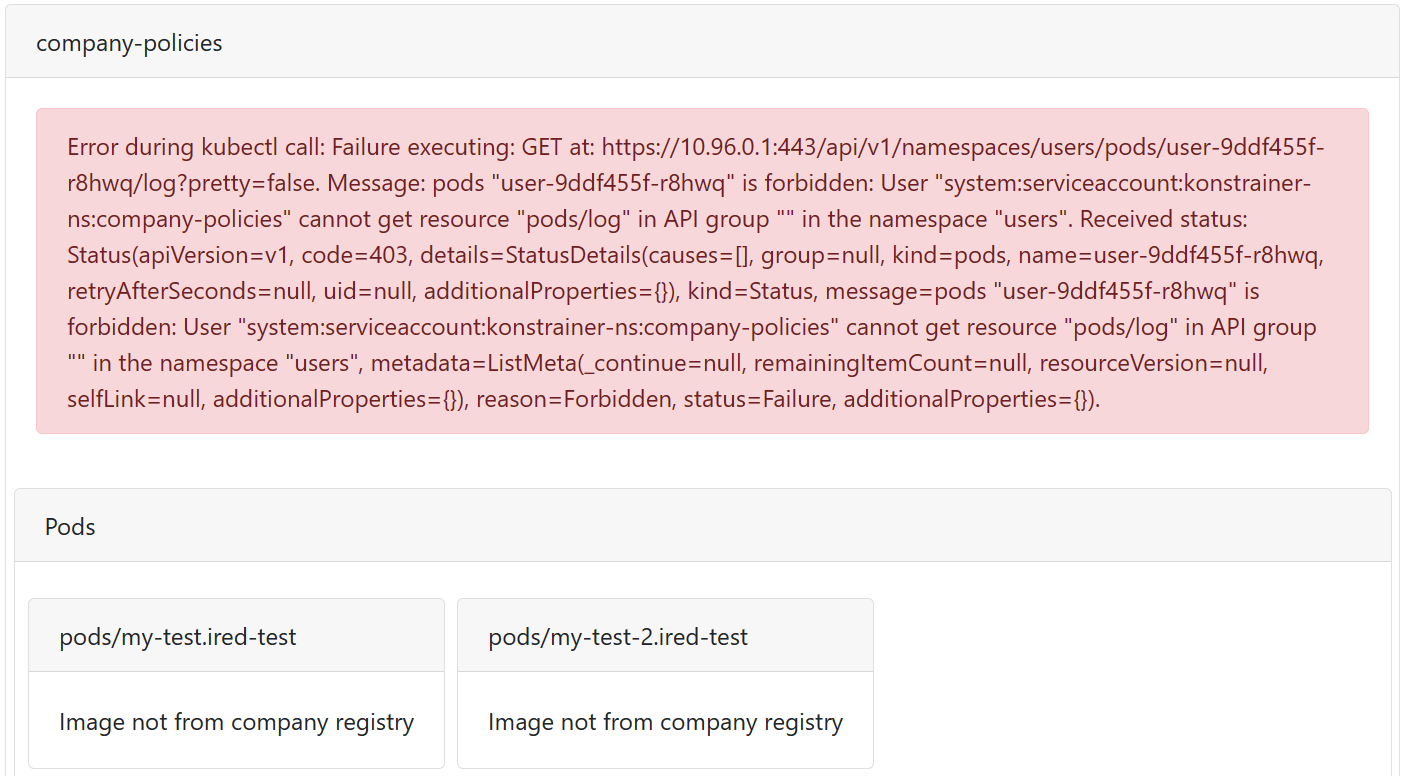
\includegraphics[width=150mm, keepaspectratio]{content/60_caseStudy2/error.png}
  \caption{Error handling in the report}
  \label{fig:report_err}
\end{figure}

We can observe an error at the top of the report, but the rest of the report still generates successfully. The cause of the error is easily identifiable by reading the error message: `Error during kubectl call: Failure executing: GET at: (...). Message: pods "user-(...)" is forbidden: User "system:serviceaccount:konstrainer-ns:company-policies" cannot get resource "pods/log" in API group "" in the namespace "users".' As a reminder, we previously configured a custom cluster role for our agent, allowing only read and list operations on pods. Since pod logs are a different resource, we need to grant the agent access to the logs as well. Changing the `clusterRole' property to `ReadAny' resolves the error.

After resolving the error, we can proceed to test the new rule. By port-forwarding a pod of the users service and attempting to log in with invalid credentials, the pod will be included in the report (after refreshing the page), tagged with the label: `Leaks secret in logs.' The steps to perform these actions are outlined in the \ref{code:c2_6} code snippet.

\begin{lstlisting}[caption={Invalid login atempt},language=bash,label=code:c2_6]
kubectl port-forward -n users pod/<pod_name> 8078:8078
# Start a new terminal
curl http://localhost:8078/login -H "Content-Type: application/json" -d '{"user": "John A. Gold", "passwd": "appels"}'
# Command output: "Invalid pass"
# Refresh the report now, to see that the pod is tagged.
\end{lstlisting}

Upon inspecting the logs using the command \lstinline|kubectl logs -n users pod/<pod_name>|, we can identify potential leakage of sensitive data: `WARNING:root:Invalid login attempt: {'user': 'John A. Gold', 'passwd': 'appels'}'

This concludes the case study where I have showcased the majority of features of my platform through various examples.
